\section{La scelta dello \stage{}}
La scelta dello \stage{} non è stata molto semplice. La decisione principale da prendere era, se scegliere un progetto interno all'azienda, o 
se momentaneamente abbandonare l'azienda per fare l'esperienza di \stage{} in un'altra.\\ 
All'inizio della mia carriera lavorativa, ho avuto l'opportunità di fare un'altro \stage{} di sei mesi e questo per me è stato di fondamentale
importanza per la mia crescita professionale.\\ Mi ha permesso di imparare tantissime cose, e di mettermi alla prova in un ambiente lavorativo
diverso da quello universitario.\\ 
Lo \stage{} per me rappresenta un'opportunità per imparare nuove tecnologie, e questa volta, come per la precedente, 
poteva essere una grande occasione. \\
Dopo aver valutato i pro e i contro, riportari in figura \ref*{fig:pro-contro}, ho deciso di rimanere in azienda, perchè siamo riusciti
a trovare un progetto interessante e stimolante, che mi ha permesso di imparare nuove tecnologie, e di mettermi alla prova.\\
\begin{figure}[!h] 
  \centering 
  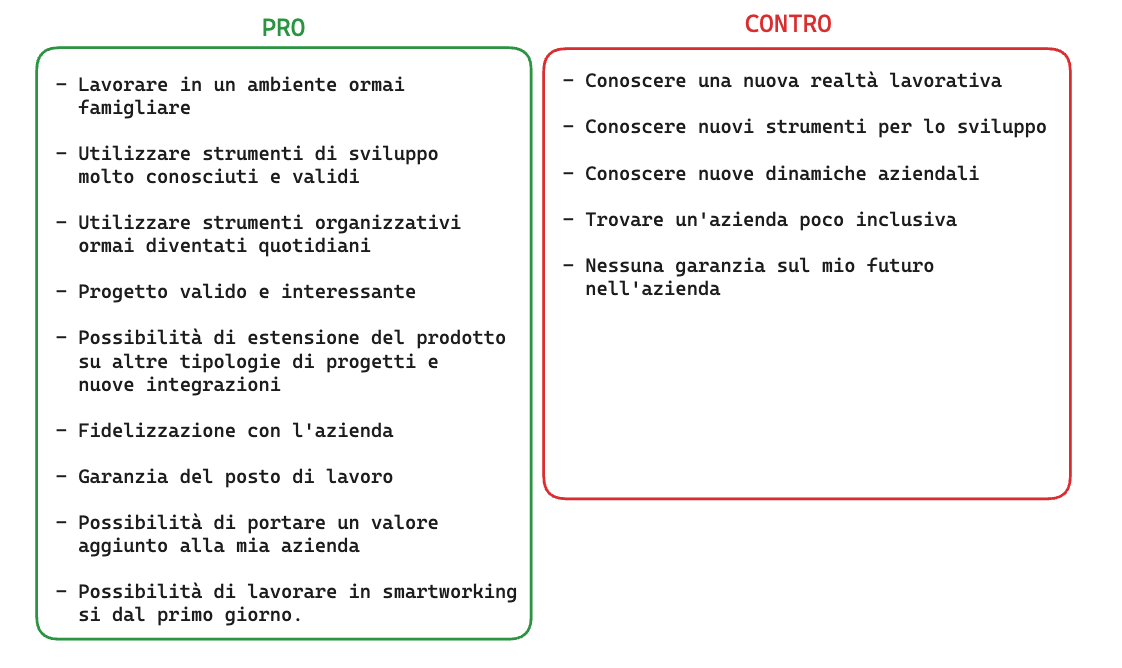
\includegraphics[width=1\columnwidth]{pro-contro.png}
  \caption{Pro e contro di fare lo \stage{} nell'azienda per cui lavoro.}
  \label{fig:pro-contro}
\end{figure}

Questo progetto mi avrebbe permesso di affrontare problemi riguardanti lo sviluppo \textit{software}, problemi di gestione e organizzazione del lavoro ma 
anche i problemi riguardanti i sistemi di \textit{build} e di \textit{continuous integration}, un argomento che mi ha sempre affascinato ma che non ho mai
avuto modo di approfondire.\\
Per questo progetto mi ero imposto degli obiettivi personali:
\begin{enumerate}
  \label{obiettivi-personali}
  \item Prendere dimestichezza con Gradle ed i sistemi di build in generale;
  \item Imparare a scrivere un \textit{plugin} per Gradle. Questo mi servirà in un futuro prossimo, per auto configurare alcuni progetto personali;
  \item Conoscere i \textit{database} a grafo, imparare ad utilizzarli e riuscire a comprendere quando è meglio utilizzarli rispetto ai \textit{database} relazionali;
  \item Provare le ultime versioni di Angular e delle librerie che solitamente uso per lo sviluppo delle \textit{web-app}; 
      In questo modo potrò valutare se è il caso di aggiornare i progetti che ho sviluppato in passato, e se è il caso di utilizzarle per i progetti futuri;
\end{enumerate}
Successivamente farò un'analisi dei risultati ottenuti, e valuterò se gli obiettivi sono stati raggiunti.\\
